% easy/easy.tex
% SPDX-License-Identifier: CC-BY-SA-3.0

\QuickQuizChapter{chp:Ease of Use}{Ease of Use}
%
\Epigraph{Creating a perfect API is like committing the perfect crime.
	  There are at least fifty things that can go wrong, and if you are
	  a genius, you might be able to anticipate twenty-five of them.}
	 {\emph{With apologies to any Kathleen Turner fans who might
	  still be alive.}}

\section{What is Easy?}
\label{sec:easy:What is Easy?}

``쉽다'' 는건 상대적인 용어입니다.
예를 들어, 많은 사람들은 15 시간의 비행을 약간 괴로운 체험일 것이라
여깁니다---그들이 대체할 수 있는 이동수단, 특히 수영과 같은 것을 고려하는 것을
멈추지 않는다면 말이죠.
이는 사용하기 편리한 API 를 만드는 것은 여러분의 의도된 사용자들을 상당히 잘
알아야 함을 의미합니다.

다음의 질문은 이 지점을 잘 설명합니다: ``오늘날 살아가는 사람들 가운데
무작위적으로 선택된 사람을 하나 놓고 생각할 때, 어떤 변경이 그의 또는 그녀의
삶을 개선시킬까요?''
\iffalse

``Easy'' is a relative term.
For example, many people would consider a 15-hour airplane flight to be
a bit of an ordeal---unless they stopped to consider alternative modes
of transportation, especially swimming.
This means that creating an easy-to-use API requires that you know
quite a bit about your intended users.

The following question illustrates this point: ``Given a randomly chosen
person among everyone alive today, what one change would
improve his or her life?''
\fi

모든 사람의 삶을 도울 것이라 보장되는 하나의 변화는 존재하지 않습니다.
무엇보다도, 굉장히 다양한 부류의 사람들이 연관된 다양한 범위의 필요, 원하는것,
소망, 그리고 열망을 가지고 존재하고 있습니다.
굶어 죽어가고 있는 사람은 음식을 필요로 할 것입니다만, 병적으로 비만인 사람에게
음식을 더 주는 것은 그의 죽음을 앞당길 수도 있습니다.
많은 젊은 사람들에 의해서 열광적으로 소망되는 높은 수준의 짜릿함은
심장마비로부터 회복되고 있는 누군가에게는 치명적일 수 있습니다.
한 사람의 성공에 중요한 정보는 너무 많은 정보의 부하로 고통받고 있는
누군가에게는 실패를 줄수도 있습니다.
짧게 말해서, 여러분이 전혀 모르는 누군가를 돕기 위한 목적의 소프트웨어
프로젝트를 위해 일하고 있다면, 여러분은 그 누군가가 여러분의 노력에 덜
감명받더라도 놀라지 않아야 합니다.
\iffalse

There is no single change that would be guaranteed to help everyone's life.
After all, there is an extremely wide range of people, with a correspondingly
wide range of needs, wants, desires, and aspirations.
A starving person might need food, but additional food might well hasten
the death of a morbidly obese person.
The high level of excitement so fervently desired by many young people
might well be fatal to someone recovering from a heart attack.
Information critical to the success of one person might contribute to
the failure of someone suffering from information overload.
In short, if you are working on a software project that is intended to
help someone you know nothing about, you should not be surprised when
that someone is less than impressed with your efforts.
\fi

여러분이 정말로 어떤 집단의 사람들을 돕고자 한다면, 그들과 일정한 기간의
시간동안 그들과 가까이 작업을 하는것을 대체할 수는 없습니다.
더도 아니고 덜도 아니고, 여러분의 사용자들이 여러분의 소프트웨어로 인해
행복해지는 정도를 늘리기 위해서 여러분이 할 수 있는 몇가지 간단한 것들이
존재하고, 그 중 일부는 다음 섹션에서 다뤄집니다.
\iffalse

If you really want to help a given group of people, there is simply no
substitute for working closely with them over an extended period of time.
Nevertheless, there are some simple things that you can do to increase
the odds of your users being happy with your software, and some of these
things are covered in the next section.
\fi

\section{Rusty Scale for API Design}
\label{sec:easy:Rusty Scale for API Design}

% Rusty is OK with this: July 19, 2006.

이 섹션은 Rusty Russell 의 2003 Ottawa Linux Symposium 키노트~\cite[Slides
39-57]{RustyRussell2003OLSkeynote} 에서 가져와졌습니다.
Rusty 의 주장의 핵심은 목표는 API 를 단순히 사용하기 편하게 만드는 게 아니라,
API 가 잘못 사용되기 어렵게 해야 한다는 것입니다.
그런 결론 하에서, Rusty 는 잘못사용하기 어렵게 하는 속성을 중요한 순서로
내림차순으로 정리한 ``Rusty Scale'' 을 제안했습니다.

다음의 리스트는 Rusty Scale 을 리눅스 커널에 일반화 시킵니다:
\iffalse

This section is adapted from portions of Rusty Russell's 2003 Ottawa Linux
Symposium keynote address~\cite[Slides 39-57]{RustyRussell2003OLSkeynote}.
Rusty's key point is that the goal should not be merely to make an API
easy to use, but rather to make the API hard to misuse.
To that end, Rusty proposed his ``Rusty Scale'' in decreasing order
of this important hard-to-misuse property.

The following list attempts to generalize the Rusty Scale beyond the
Linux kernel:
\fi

\begin{enumerate}
\item	잘못 사용되는 것은 불가능합니다.
	이건 모든 API 디자이너들이 노력해야 할 표준이긴 합니다만, 가상의 \co{dwim()}\footnote{
	\co{dwim()} 함수는 ``do what I mean (내가 의미하는걸 하라)'' 의
	약자입니다.}
	커맨드가 이를 안지킨, 잘못된 예에 가깝습니다.
\item	컴파일러나 링커는 여러분을 잘못되게 두지 않습니다.
\item	컴파일러나 링커는 여러분이 잘못한 경우에는 경고를 합니다.
\item	가장 간단한 사용법이 올바른 사용법입니다.
\item	이름은 여러분이 그걸 어떻게 사용해야 하는지 알려줘야 합니다.
\item	올바르게 사용하지 않는다면 그것은 수행시간에 항상 깨져야 합니다.
\item	일반적인 관례를 따라야 하며, 그렇게 하면 여러분은 올바른 동작을 얻게
	될겁니다.
	메모리 할당을 잘못하기는 쉽지만, 수많은 프로젝트들이 적어도 대부분의
	경우에는 메모리 할당을 올바르게 관리합니다.
	\co{malloc()} 을 Valgrind~\cite{ValgrindHomePage} 와 함께 사용하는
	행위는 \co{malloc()} 을 거의 ``올바르게 사용해야 하며, 그러지 않는다면
	수행시간에 항상 깨지는'' 지점까지 옮겨 놓을 겁니다.
\iffalse

\item	It is impossible to get wrong.
	Although this is the standard to which all API designers should
	strive, only the mythical \co{dwim()}\footnote{
		The \co{dwim()} function is an acronym that expands to
		``do what I mean''.}
	command manages to come close.
\item	The compiler or linker won't let you get it wrong.
\item	The compiler or linker will warn you if you get it wrong.
\item	The simplest use is the correct one.
\item	The name tells you how to use it.
\item	Do it right or it will always break at runtime.
\item	Follow common convention and you will get it right.
	The \co{malloc()} library function is a good example.
	Although it is easy to get memory allocation wrong, a
	great many projects do manage to get it right, at least most
	of the time.
	Using \co{malloc()} in conjunction with
	Valgrind~\cite{ValgrindHomePage} moves \co{malloc()}
	almost up to the ``do it right or it will always break at runtime''
	point on the scale.
\fi
\item	문서를 읽으면 여러분은 올바른 동작을 얻을 것입니다.
\item	구현을 들여다보면 여러분은 올바른 동작을 얻을 것입니다.
\item	올바른 메일링 리스트 기록을 읽으면 여러분은 올바른 동작을 얻을 것입니다.
\item	올바른 메일링 리스트 기록을 읽으면 여러분은 잘못된 동작을 얻을 것입니다.
\item	구현을 들여다보면 여러분은 잘못된 동작을 얻을 것입니다.
	\co{rcu_read_lock()} 의 \co{CONFIG_PREEMPT} 없을 때의 원래
	구현~\cite{PaulEMcKenney2007PreemptibleRCU} 은 이 요점의 유명하지 않은,
	하나의 예입니다.
\item	문서를 읽으면 여러분은 잘못된 동작을 얻을 것입니다.
	예를 들어, DEC Alpha \co{wmb} 인스트럭션의 문서~\cite{ALPHA95} 는 이
	인스트럭션이 실제로 하는 것에 비해 더 많이 엄격한 메모리 순서 의미를
	갖는다고 개발자들이 생각하게끔 만들었습니다.
	나중의 문서는 이 점에 대해서
	설명해서~\cite{Compaq01,WilliamPugh2000Gharachorloo}, \co{wmb}
	인스트럭션을 ``문서를 읽으면 여러분은 올바른 동작을 얻을 것입니다''
	지점으로 옮겼습니다.
\item	일반적인 관계를 따르면 여러분은 잘못된 동작을 얻을 것입니다.
	\co{printf()} 명령은 이런 요점의 한 예인데, 개발자들은 거의 항상
	\co{printf()} 의 에러 리턴을 체크하지 않기 때문입니다.
\iffalse

\item	Read the documentation and you will get it right.
\item	Read the implementation and you will get it right.
\item	Read the right mailing-list archive and you will get it right.
\item	Read the right mailing-list archive and you will get it wrong.
\item	Read the implementation and you will get it wrong.
	The original non-\co{CONFIG_PREEMPT} implementation of
	\co{rcu_read_lock()}~\cite{PaulEMcKenney2007PreemptibleRCU}
	is an infamous example of this point on the scale.
\item	Read the documentation and you will get it wrong.
	For example, the DEC Alpha \co{wmb} instruction's
	documentation~\cite{ALPHA95} fooled a
	number of developers into thinking that that this instruction
	had much stronger memory-order semantics than it actually does.
	Later documentation clarified this
	point~\cite{Compaq01,WilliamPugh2000Gharachorloo},
	moving the \co{wmb} instruction up to the
	``read the documentation and you will get it right'' point on
	the scale.
\item	Follow common convention and you will get it wrong.
	The \co{printf()} statement is an example of this point on the
	scale because
	developers almost always fail to check \co{printf()}'s error return.
\fi
\item	올바르게 수행한다면 그것은 항상 수행시점에서 깨질 겁니다.
\item	이름은 여러분이 그것을 어떻게 사용해선 안되는지 설명해 줘야 합니다.
\item	분명한 사용은 잘못된 것입니다.
	리눅스 커널의 \co{smp_mb()} 함수는 이 요점의 한 예입니다.
	많은 개발자들이 이 함수는 실제로 그것이 가지고 있는 것에 비해 강한 순서
	규칙을 가지고 있을 것이라 가정합니다.
	Section~\ref{sec:advsync:Memory Barriers} 는 이런 실수를 막기 위해
	필요한 정보를 담고 있으며, 리눅스 커널 소스 트리의 \co{Documentation}
	디렉토리 역시 그런 정보를 담고 있습니다.
\item	컴파일러나 링커는 여러분이 올바른 일을 한다면 경고를 해줄 겁니다.
\item	컴파일러나 링커는 여러분이 올바른 일을 하도록 놔두지 않을 겁니다.
\item	올바른 일을 하는 것은 중요합니다.
	\co{gets()} 함수는 이 요점의 하나의 유명한 예입니다.
	실제로, \co{gets()} 는 무조건적인 버퍼 오버플로우 보안 구멍으로 설명될
	수 있을 겁니다.
\iffalse

\item	Do it right and it will break at runtime.
\item	The name tells you how not to use it.
\item	The obvious use is wrong.
	The Linux kernel \co{smp_mb()} function is an example of
	this point on the scale.
	Many developers assume that this function has much
	stronger ordering semantics than it possesses.
	Chapter~\ref{chp:memorder:Memory Ordering} contains the
	information needed to avoid this mistake, as does the
	Linux-kernel source tree's \co{Documentation} directory.
\item	The compiler or linker will warn you if you get it right.
\item	The compiler or linker won't let you get it right.
\item	It is impossible to get right.
	The \co{gets()} function is a famous example of this point on
	the scale.
	In fact, \co{gets()} can perhaps best be described as
	an unconditional buffer-overflow security hole.
\fi
\end{enumerate}

\section{Shaving the Mandelbrot Set}
\label{sec:easy:Shaving the Mandelbrot Set}

유용한 프로그램들은
(Figure~\ref{fig:easy:Mandelbrot Set} 에 보인) Mandelbrot 집합과 깔끔하게
떨어지는 부드러운 외곽을 갖지 않는다는 점에서 닮았습니다---만약 그런 외곽을
갖는다면, halting problem 이 풀릴 수 있을 겁니다.
하지만 우린 진짜 사람이 사용할 수 있는 API 가 필요하지, 각각의 모든 잠재적
사용에 Ph.D. 학위 논문이 필요한 것들을 원하는게 아닙니다.
따라서, 우리는 ``Mandelbrot 집합을 깎아내서'',\footnote{
	Josh Triplett 덕에.}
API 의 사용을 잠재적 사용의 전체 집합 중 쉽게 설명될 수 있는 부분집합으로
제한시켜야 합니다.
\iffalse

The set of useful programs resembles the Mandelbrot set
(shown in Figure~\ref{fig:easy:Mandelbrot Set})
in that it does
not have a clear-cut smooth boundary---if it did, the halting problem
would be solvable.
But we need APIs that real people can use, not ones that require a
Ph.D. dissertation be completed for each and every potential use.
So, we ``shave the Mandelbrot set'',\footnote{
	Due to Josh Triplett.}
restricting the use of the
API to an easily described subset of the full set of potential uses.
\fi

\begin{figure}[htb]
\centering
\resizebox{3in}{!}{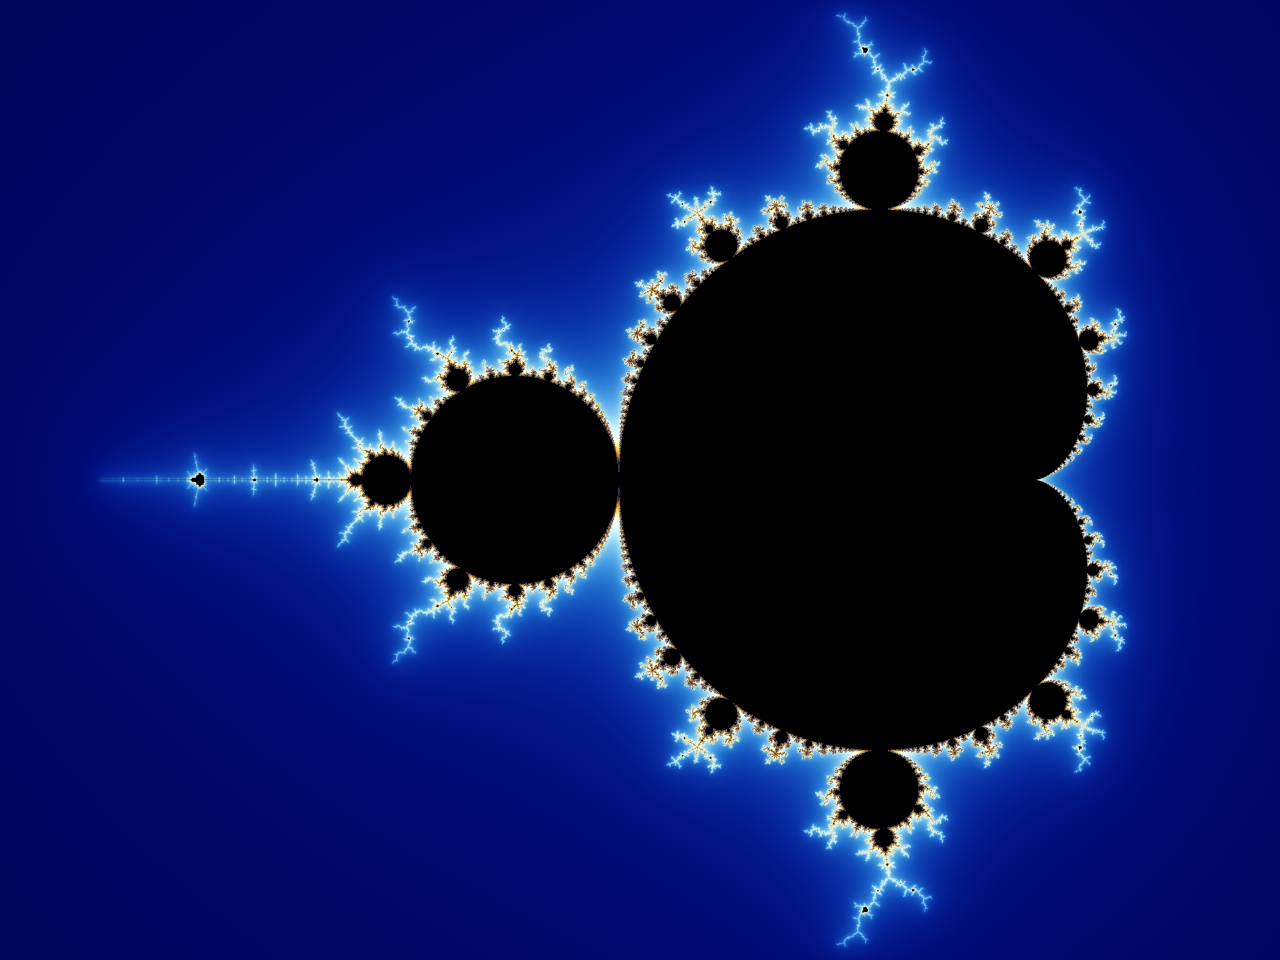
\includegraphics{easy/Mandel_zoom_00_mandelbrot_set}}
\caption{Mandelbrot Set (Courtesy of Wikipedia)}
\label{fig:easy:Mandelbrot Set}
\end{figure}

그런 깎아냄은 비생산적으로 보일 수도 있습니다.
무엇보다, 한 알고리즘이 동작한다면, 왜 그걸 사용하지 말아야 할까요?

최소한 일부의 깎아내기는 분명히 필요한 이유를 보기 위해서, 데드락을 예방하는,
하지만 가능한 가장 나쁜 방법을 사용하는 락킹 설계를 생각해 봅시다.
이 설계는 순환식 이중 링크드 리스트를 사용하는데, 이 리스트는 시스템 상의
각각의 쓰레드를 위해 하나의 헤더 원소와 함께 하나의 원소를 유지합니다.
새로운 쓰레드가 시작되면, 그 부모 쓰레드는 이 리스트에 새로운 원소를
집어넣어야만 하는데, 이는 어떠한 종류의 동기화를 필요로 합니다.

이 리스트를 보호하는 한가지 방법은 글로벌 락을 사용하는 것입니다.
하지만, 이는 쓰레드들이 빈번하게 생성되고 소멸된다면 병목지점이 될 수도
있습니다.\footnote{
	운영체제에 대한 많은 배경지식을 가지고 있는 여러분이라면, 이 말을
	불신하는 걸 잠시 멈춰주세요.
	이 말에 대한 불신을 잠시 멈추는게 불가능하다면, 우리에게 이보다 더 나은
	예를 보내주세요.}
또다른 방법은 해시 테이블을 사용하고 개별적인 hash bucket 들을 락으로 관리하는
것입니다만, 이는 리스트를 원소 순서대로 스캔할 때에는 나쁜 성능으로 동작할
겁니다.
\iffalse

Such shaving may seem counterproductive.
After all, if an algorithm works, why shouldn't it be used?

To see why at least some shaving is absolutely necessary, consider
a locking design that avoids deadlock, but in perhaps the worst possible way.
This design uses a circular doubly linked list, which contains one
element for each thread in the system along with a header element.
When a new thread is spawned, the parent thread must insert a new
element into this list, which requires some sort of synchronization.

One way to protect the list is to use a global lock.
However, this might be a bottleneck if threads were being created and
deleted frequently.\footnote{
	Those of you with strong operating-system backgrounds, please
	suspend disbelief.
	If you are unable to suspend disbelief, send us a better example.}
Another approach would be to use a hash table and to lock the individual
hash buckets, but this can perform poorly when scanning the list in order.
\fi

세번째 방법은 개별의 리스트 원소들을 락으로 보호하고, 원소의 삽입 시에 해당
원소의 앞쪽 원소와 뒤쪽 원소 둘 다의 락을 잡는 겁니다.
두 락이 모두 잡혀야 하므로, 그것들을 어떤 순서로 잡을 것인지를 우리는 결정해야
합니다.
그런 두개의 일반적인 방법은 락들을 주소순서로 잡거나 그것들이 리스트에 보여지는
순서대로 잡아서, 락으로 잠겨지는 두개의 원소 중 하나가 잠겨질 때 그 헤더가 항상
먼저 얻어지도록 하는 것입니다.
하지만, 이 방법들 모두 특별한 경우 검사와 분기를 필요로 합니다.

여기서 깎아내져야 하는 해결책은 락들을 무조건적으로 리스트 순서로 잡는
것입니다.
하지만 데드락은 어떡하죠?

데드락은 일어날 수 없습니다.
\iffalse

A third approach is to lock the individual list elements, and to require
the locks for both the predecessor and successor to be held during the
insertion.
Since both locks must be acquired, we need to decide which order to
acquire them in.
Two conventional approaches would be to acquire the locks in address
order, or to acquire them in the order that they appear in the list,
so that the header is always acquired first when it is one of the two
elements being locked.
However, both of these methods require special checks and branches.

The to-be-shaven solution is to unconditionally acquire the locks in
list order.
But what about deadlock?

Deadlock cannot occur.
\fi

이를 알아보기 위해, 리스트의 원소를 헤더를 0으로, (순환형 리스트이므로, 헤더의
앞쪽 원소인) 리스트의 마지막 원소를 $N$ 으로 하는식으로 번호를 매깁시다.
비슷하게, 쓰레드들을 0부터 $N-1$ 까지로 번호매깁시다.
만약 각각의 쓰레드가 원소들 가운데 연속적인 두개의 원소들의 락을 잡으려 한다면,
최소한 하나의 쓰레드는 두 락들을 모두 잡을 수 있도록 보장될 겁니다.

왜죠?

리스트의 모든 것들에 닿을 만큼 쓰레드들의 수가 충분히 많지 않기 때문입니다.
쓰레드~0 가 원소~0 의 락을 잡는다고 생각해 봅시다.
이 쓰레드가 블락되기 위해서는, 어떤 다른 쓰레드가 이미 원소~1 의 락을 잡았어야
하는데, 쓰레드~1이 그러고 있다고 가정해 봅시다.
비슷하게, 쓰레드~1 이 블락되기 위해서는 어떤 다른 쓰레드가 원소~2 의 락을 잡고
있어야 하는데, 이런식으로 쓰레드~$N-1$ 까지 연속되는데, 이 쓰레드는 원소~$N-1$
의 락을 획득합니다.
쓰레드~$N-1$ 이 블락되기 위해서는 어떤 다른 쓰레드가 원소~$N$ 의 락을 잡고
있어야 합니다.
하지만 더이상 쓰레드가 존재하지 않고, 따라서 쓰레드~$N-1$ 은 블락될 수가
없습니다.
따라서, 데드락은 일어나지 않습니다.
\iffalse

To see this, number the elements in the list starting with zero for the
header up to $N$ for the last element in the list (the one preceding the
header, given that the list is circular).
Similarly, number the threads from zero to $N-1$.
If each thread attempts to lock some consecutive pair of elements,
at least one of the threads is guaranteed to be able to acquire both
locks.

Why?

Because there are not enough threads to reach all the way around the list.
Suppose thread~0 acquires element~0's lock.
To be blocked, some other thread must have already acquired element~1's
lock, so let us assume that thread~1 has done so.
Similarly, for thread~1 to be blocked, some other thread must have acquired
element~2's lock, and so on, up through thread~$N-1$, who acquires
element~$N-1$'s lock.
For thread~$N-1$ to be blocked, some other thread must have acquired
element~$N$'s lock.
But there are no more threads, and so thread~$N-1$ cannot be blocked.
Therefore, deadlock cannot occur.
\fi

그러니 우리가 왜 이 마음에 드는 작은 알고리즘의 사용을 막아야 합니까?

여러분이 \emph{정말로} 그걸 사용하고자 한다면, 우리는 여러분을 막을 수 없는게
사실입니다.
하지만, 우리는 우리가 신경쓰는 어떤 프로젝트에도 그런 코드가 들어오지 못하도록
추천할 수 \emph{있습니다}.

하지만, 여러분이 이 알고리즘을 사용하기 전에, 다음의 Quick Quiz 를 한번 생각해
주시기 바랍니다.
\iffalse

So why should we prohibit use of this delightful little algorithm?

The fact is that if you \emph{really} want to use it, we cannot stop you.
We \emph{can}, however, recommend against such code being included
in any project that we care about.

But, before you use this algorithm, please think through the following
Quick Quiz.
\fi

\QuickQuiz{}
	원소를 지울 때에도 비슷한 알고리즘을 사용할 수 있습니까?
	\iffalse

	Can a similar algorithm be used when deleting elements?
	\fi
\QuickQuizAnswer{
	네.
	하지만, 각각의 쓰레드는 가운데 하나를 삭제하기 위해 연속된 세개의
	원소의 락을 잡아야 하므로, $N$ 개의 쓰레드가 존재한다면, 데드락이
	없도록 하기 위해서는 리스트에 ($N+1$ 개가 아니라) $2N+1$ 개의 원소가
	존재해야만 합니다.
	\iffalse

	Yes.
	However, since each thread must hold the locks of three
	consecutive elements to delete the middle one, if there
	are $N$ threads, there must be $2N+1$ elements (rather than
	just $N+1$) in order to avoid deadlock.
	\fi
} \QuickQuizEnd

이 알고리즘은 극도로 특수화 되어 있으며 (이 알고리즘은 특수한 크기의 리스트에
대해서만 동작합니다), 또한 상당히 취약한 게 사실입니다.
리스트에 노드를 하나 추가하는데 의도치 않게 실패하게 하는 어떤 버그든 데드락을
초래할 수 있습니다.
사실, 노드를 약간이라도 너무 늦게 추가하는 것만으로도 데드락을 초래할 수
있습니다.

또한, 앞에서 설명한 다른 알고리즘들이 ``좋고 충분합니다''.
예를 들어, 단순히 락들을 주소 순서대로 잡는 것은 상당히 간단하고 빠르면서도
어떤 크기의 리스트든 사용할 수 있게 합니다.
다만 비어있는 리스트와 하나의 원소만을 포함하고 있는 리스트의 특수한 경우들에
대해서만 조심하세요!
\iffalse

The fact is that this algorithm is extremely specialized (it only works
on certain sized lists), and also quite fragile.
Any bug that accidentally failed to add a node to the list could result
in deadlock.
In fact, simply adding the node a bit too late could result in deadlock.

In addition, the other algorithms described above are ``good and sufficient''.
For example, simply acquiring the locks in address order is fairly simple
and quick, while allowing the use of lists of any size.
Just be careful of the special cases presented by empty lists and lists
containing only one element!
\fi

\QuickQuiz{}
	그러쿤요!
	이처럼 깎여져나갈 가치가 있는 알고리즘을 가지고 나타난 누군가를 포용해
	본 적 있나요???
	\iffalse

	Yetch!
	What ever possessed someone to come up with an algorithm
	that deserves to be shaved as much as this one does???
	\fi
\QuickQuizAnswer{
	그건 Paul 일 수 있을 겁니다.

	그는 다섯명의 철학자들이 참가하는 비위생적인 스파게티 저녁식사에
	관련된, \emph{Dining Philosopher's Problem} 을 생각하고 있었습니다.
	다섯개의 접시가 있지만 다섯개의 포크만이 테이블에 있다는 점을 가지고,
	그리고 각각의 철학자는 식사를 위해 한번에 두개의 포크가 필요하다는 점을
	가지고, 누군가는 데드락을 예방하는 포크 할당 알고리즘을 생각해 낼 수
	있을 겁니다.
	Paul 의 응답은 ``조용!  그냥 다섯개 더 포크를 가져와!'' 였습니다.

	이건 그 자체로는 괜찮습니다만, Paul 은 이내 이와 똑같은 해결책을 순환형
	링크드 리스트에 적용했습니다.

	이것 역시 그렇게 나쁘진 않았을 겁니다만, 그는 누군가에게 그에 대해
	이야기를 해야만 했습니다!
	\iffalse

	That would be Paul.

	He was considering the \emph{Dining Philosopher's Problem}, which
	involves a rather unsanitary spaghetti dinner attended by
	five philosophers.
	Given that there are five plates and but five forks on the table, and
	given that each philosopher requires two forks at a time to eat,
	one is supposed to come up with a fork-allocation algorithm that
	avoids deadlock.
	Paul's response was ``Sheesh!  Just get five more forks!''

	This in itself was OK, but Paul then applied this same solution to
	circular linked lists.

	This would not have been so bad either, but he had to go and tell
	someone about it!
	\fi
} \QuickQuizEnd

정리하자면, 우린 그저 동작한다는 이유만으로 알고리즘을 사용하지는 않습니다.
그대신에 우리는 배울 가치가 충분한 알고리즘들만 사용하도록 우리 자신을
제한합니다.
더 어렵고 더 복잡한 알고리즘일수록, 그걸 배우고 그 버그를 고치는데 드는 고통이
가치가 있을 수 있도록 더 일반적으로 유용해야만 합니다.
\iffalse

In summary, we do not use algorithms simply because they happen to work.
We instead restrict ourselves to algorithms that are useful enough to
make it worthwhile learning about them.
The more difficult and complex the algorithm, the more generally useful
it must be in order for the pain of learning it and fixing its bugs to
be worthwhile.
\fi

\QuickQuiz{}
	이 규칙에 대한 예외를 대 보세요.
	\iffalse

	Give an exception to this rule.
	\fi
\QuickQuizAnswer{
	한가지 예외는 주어진 상황 하에서는 유일하게 동작하는 어렵고 복잡한
	알고리즘이 될 수 있을 겁니다.
	또다른 예외는 주어진 상황에서 동작하는 것으로 알려진 것 중에서는 가장
	간단한, 어렵고 복잡한 알고리즘이 될 수 있을 겁니다.
	하지만, 이런 경우들에 있어서조차도, 더 간단한 알고리즘을 내놓기 위해
	조금 시간을 써보는게 좋을 겁니다!
	무엇보다도, 여러분이 어떤 작업을 하는 첫번째 알고리즘을 만들어내게
	된다면, 더 간단한 것을 하나 만드는 것은 그렇게까지 어렵지는 않을
	겁니다.
	\iffalse

	One exception would be a difficult and complex algorithm that
	was the only one known to work in a given situation.
	Another exception would be a difficult and complex algorithm
	that was nonetheless the simplest of the set known to work in
	a given situation.
	However, even in these cases, it may be very worthwhile to spend
	a little time trying to come up with a simpler algorithm!
	After all, if you managed to invent the first algorithm
	to do some task, it shouldn't be that hard to go on to
	invent a simpler one.
	\fi
} \QuickQuizEnd

예외는 차치하고, 우리는 우리의 프로그램들이
Figure~\ref{fig:easy:Shaving the Mandelbrot Set}
에 보여진 것처럼 유지가능한 상태를 유지할 수 있도록 소프트웨어를 깎아내기를
계속해야만 합니다.
\iffalse

Exceptions aside, we must continue to shave the software ``Mandelbrot
set'' so that our programs remain maintainable, as shown in
Figure~\ref{fig:easy:Shaving the Mandelbrot Set}.
\fi

\begin{figure}[htb]
\centering
\resizebox{3in}{!}{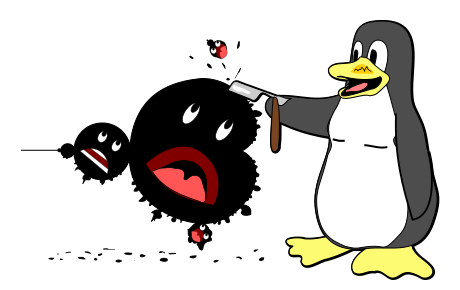
\includegraphics{cartoons/r-2014-shaving-the-mandelbrot}}
\caption{Shaving the Mandelbrot Set}
\ContributedBy{Figure}{fig:easy:Shaving the Mandelbrot Set}{Melissa Broussard}
\end{figure}
